\documentclass[9pt,a4paper]{extarticle}

\usepackage{f1000_styles}

\usepackage{hyperref}

\usepackage[numbers]{natbib}

% include \verb macros in \caption of figures

% http://tex.stackexchange.com/a/8814

\usepackage{cprotect}

\begin{document}

\pagestyle{front}

\title{Creating and sharing reproducible research code the workflowr
way}

\author[1]{John D. Blischak}

\author[1,2]{Peter Carbonetto}

\author[1,3]{Matthew Stephens}

\affil[1]{Department of Human Genetics, University of Chicago}

\affil[2]{Research Computing Center, University of Chicago}

\affil[3]{Department of Statistics, University of Chicago}

\maketitle

\thispagestyle{front}

\begin{abstract}

\# Note: Abstract can be as long as 300 words.

The workflowr R package helps scientists create code and results that
are organized, reproducible, well-documented, and more effectively
communicated with other scientists. Workflowr provides a core set of
commands that are easily integrated into research practice to make
analyses more reproducible and accessible. The core workflowr commands
implement four key features of reproducible code: (1) an automatic
project structure that promotes better organization of data, code and
results; (2) code and results that are packaged together, and
incorporated into a project development history; (3) "reproducibility
checks" that accompany each packaged collection of code and results; and
(4) tools to facilitate online sharing of project code and results. To
achieve these reproducibility features, workflowr integrates version
control (Git), literate programming tools (knitr, R Markdown), and
static website hosting (e.g., GitHub Pages) into a simple, uniform
interface in R. Our aim is to encourage all scientists, regardless of
background, to develop reproducible research code, and share it. The
workflowr R package is open source and available on CRAN, with full
documentation and source code available at
https://github.com/jdblischak/workflowr.

\end{abstract}

\section*{Keywords}

reproducibility, open science, workflow, R, interactive programming,
literate programming, version control

\clearpage

\pagestyle{main}


\section*{Introduction}

A central tenet of the scientific method is that results should be
independently verifiable --- and, ideally, extendible --- by other
researchers. As computational methods play an increasing role in many
disciplines, key scientific results are often produced by computer code.
Verifying and extending such results requires that the code be
``reproducible''; that is, it can be accessed and run, with outputs that
can be corroborated against published results \cite{Buckheit1995,
Gentleman2005, Peng2011, Ince2012, Morin2012, Sandve2013,
Easterbrook2014, Stodden2016, Lowndes2017}. Unfortunately, this ideal is
not usually achieved in practice; most scientific articles do not come
with code that can reproduce their results \cite{Ioannidis2009,
Ioannidis2014, Stodden2018}.

There are many barriers to sharing reproducible code and corresponding
computational results. One barrier is simply that keeping code and
results sufficiently organized and documented is difficult --- it is
burdensome even for experienced programmers who are well-trained in
relevant computational tools such as version control (discussed later),
and even harder for the many domain scientists who write code with
little formal training in computing and informatics \cite{Wilson2014}.
Further, modern interactive computer environments (e.g., R, python),
while greatly enhancing code development \cite{Findler2002}, also make
it easier to create results that are irreducible. To take one example,
it is all too easy to run interactive code without recording or
controlling the seed of a pseudo-random number generator, or generate
results in a ``contaminated'' environment that contains objects whose
values are critical but unrecorded. Both these issues can lead to
results that are difficult or impossible to reproduce. Finally, even
when analysts produce code that is reproducible in principle, sharing it
in a way that makes it easy for others to retrieve and use (e.g., via
GitHub or Bitbucket) involves technologies that many scientists are not
familiar with \cite{Marwick2017, Stodden2018}.

In light of this, there is a pressing need for easy-to-use tools to help
analysts maintain reproducible code, document progress, and disseminate
code and results to collaborators, and to the scientific community. We
have developed an open source R \cite{R2019} package, "workflowr", to
address this need. The workflowr package aims to instill a particular
"workflow" --- a sequence of steps to be repeated and integrated into
research practice --- that helps make projects more reproducible and
accessible. To achieve this, workflowr integrates four key features that
facilitate reproducible code development: (1) version control
\cite{Loeliger2012, Chacon2014}; (2) literate programming
\cite{Xie2018}; (3) simple automated checks such as setting and
recording the random number seed that improve code reproducibility,
which we call "reproducibility safeguards"; and (4) sharing code and
results via a browsable website. These features exploit powerful
existing tools, whose mastery would take considerable study. However,
the workflowr interface is designed to be simple so that learning it
does not become another barrier in itself, and novice users can quickly
enjoy its many benefits. By simply following the "workflowr workflow", R
users can create projects whose results and figures are easily
accessible on a static website --- thereby conveniently shareable with
collaborators by sending them a URL --- and accompanied by source code
and reproducibility safeguards. The Web-based interface, updated with
version control, also makes it easy to navigate through different parts
of the project and browse the project history, including previous
versions of figures and results, and the code used to produce them. When
using workflowr, all this can be achieved with minimal experience in
version control systems and Web technologies.

The workflowr package builds on several software technologies and R
packages, without which this work would have been impossible. First,
workflowr builds on the invaluable R literate programming system
provided by knitr \cite{Xie2014, knitr} and R Markdown \cite{Xie2018,
rmarkdown}, which in turn build on pandoc, the "Markdown" markup
language, and various Web technologies such as Cascading Style Sheets
and Bootstrap \cite{Spurlock2013}. Several popular R packages extend
knitr and rmarkdown for specific uses such as writing blogs (blogdown),
monographs (bookdown) and software documentation (pkgdown). Analogously,
workflowr augments rmarkdown with additional features such as the
reproducibility safeguards, and adds integration with Git. Git was
designed to support large-scale, distributed software development, but
in workflowr it serves a different purpose: to record, and provide
access to, the development history of a project. Workflowr also uses
another Git feature, "remotes", to enable collaborative project
development across multiple locations, and to help users create
browsable projects via integrations with popular online services such as
GitHub Pages and GitLab Pages. These features are implemented using the
R package git2r, which provides an interface to the libgit2 C library.
Finally, beyond extending the R programming language, workflowr is also
integrated seamlessly with the popular RStudio interactive development
environment.

In addition to the tools upon which workflowr directly builds, there are
many other related tools that directly or indirectly advance open and
reproducible data analysis. A comprehensive review of such tools is
beyond the scope of this article, but we note that many of these tools
are complementary to workflowr in that they tackle aspects of
reproducibility that workflowr currently leaves to the user, such as:
management and deployment of computational environments and dependencies
(e.g., conda, Homebrew, Singularity, Docker, Kubernetes, packrat,
checkpoint, switchr, RSuite ~~ActivePapers
\url{https://www.activepapers.org/}~~); development and management of
computational pipelines (e.g., GNU Make, Snakemake, drake); management
and archival of data objects (e.g., archivist, cacher, Dryad, Zenodo);
and distribution of open source software (e.g., CRAN, Bioconductor,
Bioconda). Most of these tools or services could be used in combination
with workflowr. There are additional, very ambitious efforts to develop
cloud-based services that come with many computational reproducibility
features (e.g., Code Ocean, Binder, Gigantum, The Whole Tale). Many of
these platforms manage individual projects as Git repositories, so
workflowr could, in principle, be installed and used on these platforms,
possibly to enhance their existing features. Other R packages with
utilities to facilitate reproducibility that could complement workflowr
include ProjectTemplate, rrtools and usethis, as well as many of the R
packages listed in the "Reproducible Research" CRAN Task View
(https://CRAN.R-project.org/view=ReproducibleResearch) and our own
(unofficial) Task View on "Project Workflows"
(https://github.com/jdblischak/ctv-project-workflows).

Of the available software tools facilitating reproducible research,
perhaps the closest in scope to workflowr are the R package adapr
\cite{Gelfond2018} and the Python-based toolkit Sumatra
\cite{Davidson2014}. Like workflowr, both adapr and Sumatra use version
control to maintain a project development history. Unlike workflowr,
both place considerable emphasis on managing and keeping track of
dependencies (software and data), whereas workflowr only records this
information. In contrast, workflowr places more emphasis on literate
programming --- the publishing of text and code in a readable form ---
and more closely integrates other features such as tracking project
development history via Git with literate programming.

The workflowr R package is available from CRAN
(https://cran.r-project.org/package=workflowr) and GitHub
(https://github.com/jdblischak/workflowr), and is distributed under the
flexible open source MIT license. Extensive documentation, tutorials and
user support can be found at the GitHub site. In the remainder of this
article, we describe the workflowr interface, explain its design, and
give examples illustrating how workflowr is used in practice (see "Use
Cases").


\section*{Methods}

The workflowr R package makes data analysis projects more organized,
tracked, reproducible, and shareable. The R package and its dependencies
are straightforward to install, while also being highly customizable for
more dedicated users. In the following sections, we give an overview of
the features of the workflowr R package, and describe their
implementation. For step-by-step instructions on starting a workflowr
project, see the
\href{https://jdblischak.github.io/workflowr/articles/wflow-01-getting-started.html}{"Getting
started with workflowr"} vignette.

\subsection*{Operation}

For basic usage, only five functions are needed:

• \verb|wflow_start()| initializes a new project, including the template
directory structure (Figure 1A);

• \verb|wflow_build()| renders the webpages from the R Markdown analysis files,
withreproducibility safeguards in place;

• \verb|wflow_publish()| commits the rendered webpages --- and the code that
generated these webpages --- to the project development history;

• \verb|wflow_status()| is used to check the status of the project files; and

• \verb|wflow_git_push()| uploads the results from the user's local repository
to a website hosting service.

\textit{The primary output of workflowr is a project website for
browsing the results generated by the R Markdown analyses} (Figure 1B).
The project website allows for hyperlinks between related results pages,
and for a table of contents giving an overview of the results. While the
benefits of hypertext—documents that are are interconnected by
hyperlinks—are self-evident, we believe the benefits in the context of
organizing work on a scientificproject remain underappreciated. The
links improve organization and accessibility by allowing readers to
quickly navigate the different parts of the analysis (Figure \ref{fig:organized}B, and see
the Use Cases for examples). The Markdown syntax supports links using a
simple square brackets notation, so links can be easily added to the R
Markdown source files.

\subsubsection*{Organizing the project: \verb|wflow_start()|}



\begin{figure}

\# Figure \ref{fig:organized}

\centering

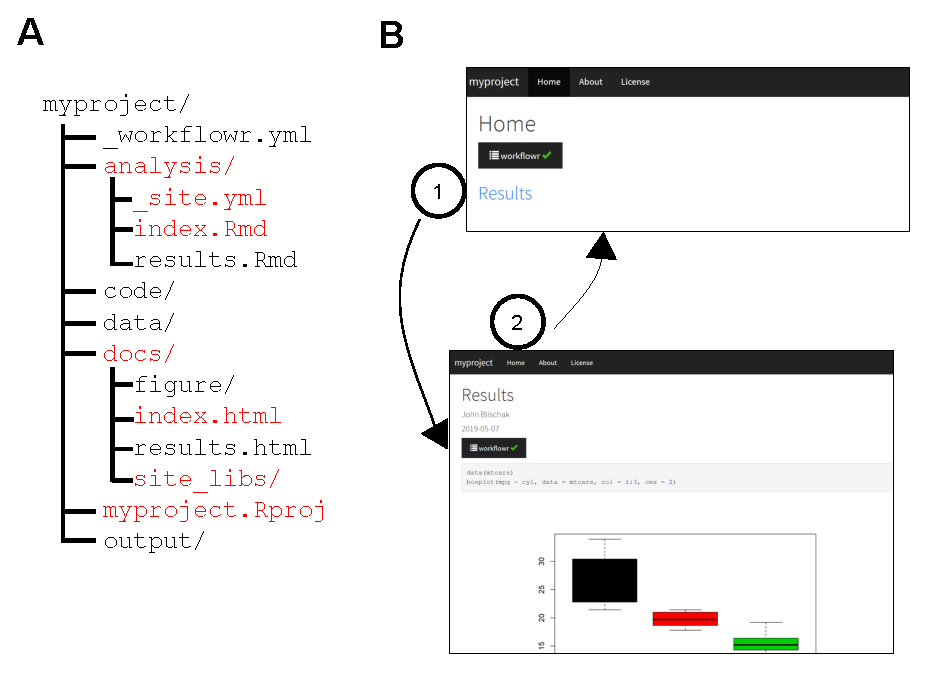
\includegraphics[width=0.8\textwidth]{figures/wflow-fig-1-v01.eps}

\cprotect\caption{\label{fig:organized}

The workflowr package helps organize files and results. A) The function
\verb|wflow_start()| populates a ~~new~~ project directory with all the files
needed to begin a workflowr project. The default directory structure
encourages users to organize their files as the project progresses.
(This is only a suggested structure, and users may change the names of
many of these files and directories later on.) Files required by
workflowr are depicted in red. B) All results are organized into a
website which is stored within the project directory, inside the "docs"
folder. The use of hyperlinks allows for efficient access of the
results. The example screenshots illustrate how a workflowr website can
be navigated. Clicking a hyperlink in the main page (1) navigates the
browser to a webpage containing some results; clicking on the "Home"
hyperlink (2) in the navigation bar brings the browser back to the main
page.

}

\end{figure}

The function \verb|wflow_start()| facilitates project organization by
populating a ~~new~~ directory with suggested subdirectories, scripts,
and configuration files for a data analysis project (Figure \ref{fig:organized}A). The
subdirectories include by default: analysis/ , where the R Markdown
analysis files are stored; docs/, which stores the workflowr website
HTML files; code/, containing longer-running scripts, compiled code
(e.g., C++) and other source code supporting the data analyses; data/,
for storing raw data files; and output/ for saving processed data files
and other outputs generated by the scripts and analyses. This setup is
flexible and configurable; only two of these directories,
\verb|analysis/| and \verb|docs/|, are required, and both can be renamed
later.

\subsubsection*{Generating the results reproducibly: \verb|wflow_build()|}

In a workflowr project, all computations are performed within the R
Markdown literate programming system \cite{Xie2018}. The user develops
their R code inside R markdown files in the analysis directory, then
calls \verb|wflow_build()|, which runs the code. This function also compiles,
or "knits", the code and results as a webpage, which is then saved to
the docs directory. The \verb|wflow_build()| function extends the \verb|render()|
command from the rmarkdown package with several reproducibility
safeguards (Figure \ref{fig:reproducible}). First, it creates a new, empty R session for
excuting the code. This is critical for reproducibility, as the results
should not depend on the current state of the user's R environment; all
objects necessary to run the code should be defined in the code, or
loaded by packages. Second, to prevent one of the most common failures
to reproduce in R—not setting the working directory before running the R
script, resulting in incorrectly resolved relative file paths—workflowr
automatically sets the working directory in a consistent manner (the
exact setting can be controlled by a workflowr configuration file; see
below). Third, it sets a seed for the pseudorandom number generator
before execution so that analyses that use random numbers always return
the same result. Fourth, it records information about the computing
environment, including the operating system and the versions of R and
packages that were used to produce the results. Finally, \verb|wflow_build()|
performs reproducibility checks and inserts a report summarizing these
checks at the top of the webpage. As long as the automatic safeguards
are not disabled by the user, each analysis will pass these checks.

\subsubsection*{Keeping track of the project's development: \verb|wflow_publish()|}

As a project progresses, many versions of the results will be generated
as results are scrutinized, analyses are revised, errors are corrected,
and new data are considered. Keeping track of a project's evolution is
important for documenting progress and retracing the development of the
analyses. This is sometimes done without version control tools by
copying code and results whenever an important change is made. This
typically results in a large collection of files with names such as
\verb|results-v2-final_final.pdf| and
\verb|anova_analyses_before_adding_new_samples.R|. This is not only
tedious, but also likely to result in errors, and makes it difficult to
communicate changes to collaborators.

Git provides a more systematic and reliable way to keep track of a
project's development history. Using Git, however, brings two new
challenges. First, since Git was originally designed for software
engineers to collaborate on large-scale software projects, the features
and documentation are far too complex for most researchers. This large
barrier to entry can discourage researchers from using Git for their
projects. Second, Git was originally intended to manage source code for
software, not for a data analysis project --- consider that the analyst
will want to track the source code and data as well as the results that
are generated by the code and data.

The \verb|wflow_publish()| function is designed precisely for these aims: it
adapts Git for use in an analysis project, while hiding the technical
aspects of calling Git. The command performs three key steps, which are
illustrated in Figure \ref{fig:publish}:

1. Commit source: Commit the R Markdown source file to the Git
repository, and record the "Secure Hash Function" --- a hexadecimal
sequence, often abbreviated as "SHA1", that uniquely identifies the
commit in the Git repository.

2. Render results: Use \verb|wflow_build()| to execute the source code, and
compile the code and results into a webpage accompanied with the
workflowr reproducibilty safeguards. The SHA1 generated in Step 1 is
also embedded into the results webpapage.

3. Commit results: Commit the webpage ~~and figure files~~ generated in
Step 2.

This three-step procedure guarantees that each new collection of results
added to the project development history has been produced by a unique
and identifiable version of an R Markdown source file.

Although we have emphasized the accessibility of workflowr to those with
little experience with Git, experienced Git users can also benefit from
using \verb|wflow_publish()| instead of running the individual R and Git
commands. Besides the convenience of running a single function,
\verb|wflow_publish()| automates implementation of these two Best Practices:

1. Every commit to an (R Markdown) analysis file is associated with a
commit to the results file generated by that analysis file.

2. \textit{An analysis file is only committed if it runs successfully};
on failure, \verb|wflow_publish()| aborts, and neither code nor results are
committed to the Git repository. Although Steps 1–3 can be replicated by
running the individual commands in R and Git, only running these steps
jointly through \verb|wflow_publish()| can guarantee that each commited results
file is accompanied by a committed, runnable source code file that can
be used to re-generate the results. (R code that does not work can still
be committed, but it will not be associated with a committed results
file containing a workflowr report.)



\begin{figure}

\# Figure \ref{fig:publish}

\centering

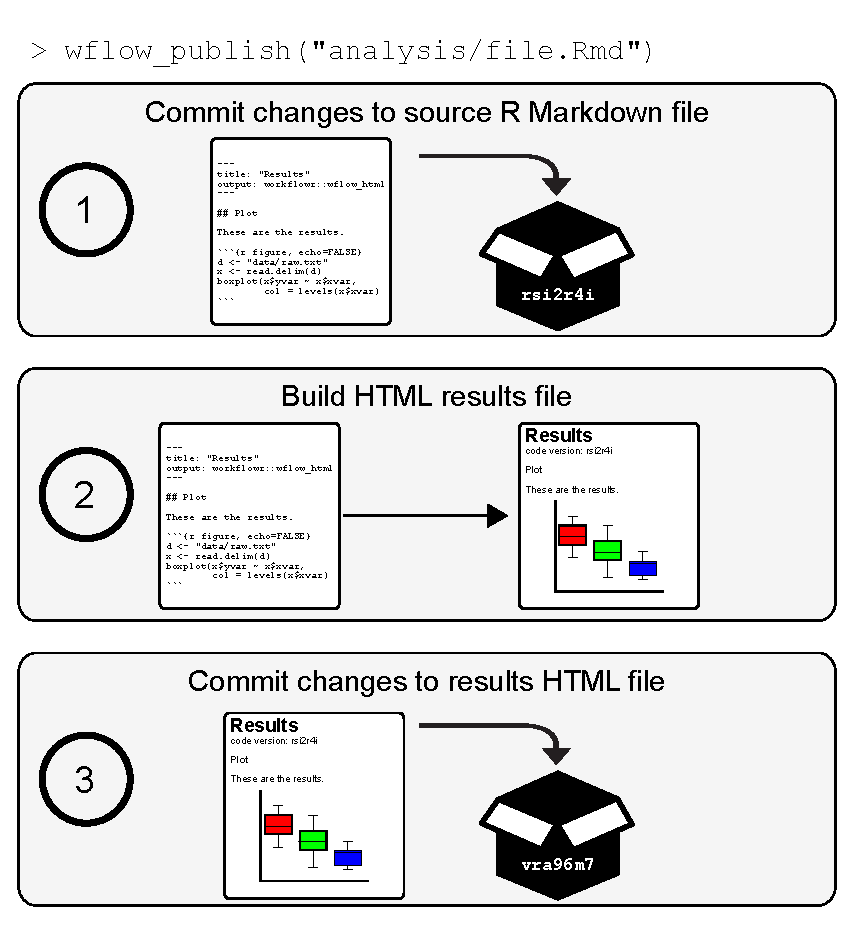
\includegraphics[width=0.8\textwidth]{figures/wflow-fig-2-v02.eps}

\cprotect\caption{\label{fig:publish}

The function \verb|wflow_publish()| versions the source and results files. The
function \verb|wflow_publish()| performs a 3-step procedure to ensure that the
result HTML file is always created from a unique and identifiable
version of the R Markdown source. (1) The first step commits the changes
to the source R Markdown file. (2) The second step builds the results
HTML file from the R Markdown source. This ensures that the results were
generated from this exact version of the R Markdown file. Furthermore,
the unique version of the Git repository is inserted directly into the
HTML file so that the source code used to generate the results is easily
identified and accessed. (3) The results HTML file (and any related
figure files) is committed to the Git repository. Thus, the results of
the analysis are versioned in addition to the source code.

}

\end{figure}

Publication of an analysis is not final --- after calling
\verb|wflow_publish()|, the analysis can be repeatedly updated and re-published
using \verb|wflow_publish()|. Each time \verb|wflow_publish()| succeeds in committing
a new version of the code and results, a link to previously published
versions of the analysis are embedded in the webpage so that readers can
quickly access previous versions and compare with the latest results.

\subsubsection*{Checking in on the project's development: \verb|wflow_status()|}

As a workflowr project grows, it is important to be able to quickly get
an overview of the project's status. This overview is provided by the
\verb|wflow_status()| command, which gives the status of each R Markdown file
in the project (Figure \ref{fig:versioned}). The status of each R Markdown file is
determined by Git --- precisely, by the the state of the file in the Git
repository's working tree, as well as the state of the corresponding
HTML file. An R Markdown file in the ``scratch'' state is a file that is
not yet tracked by Git, and therefore is not currently included in the
project development history. An ``unpublished'' R Markdown file is a
file that is being tracked by Git, but its accompanying HTML file is
not. An R Markdown file that is ``published'' is currently tracked by
Git, and its accompanying HTML file is also tracked. Once
\verb|wflow_publish()| completes successfully, the R Markdown file
automatically enters the ``published'' state.

Each R Markdown file that is in the ``published'' state is also assigned
a substatus. If no changes have been made to the R Markdown file since
its HTML file was last published, it is marked as being ``up-to-date''.
Conversely, if the R Markdown file has been modified since the last time
its HTML file was published, it is in a ``modified'' state. The
\verb|wflow_status()| function highlights all R Markdown files in the
``scratch'', ``unpublished'' or ``modified'' states and suggests steps
for updating the results using \verb|wflow_publish()|.



\begin{figure}

\# Figure \ref{fig:versioned}

\centering

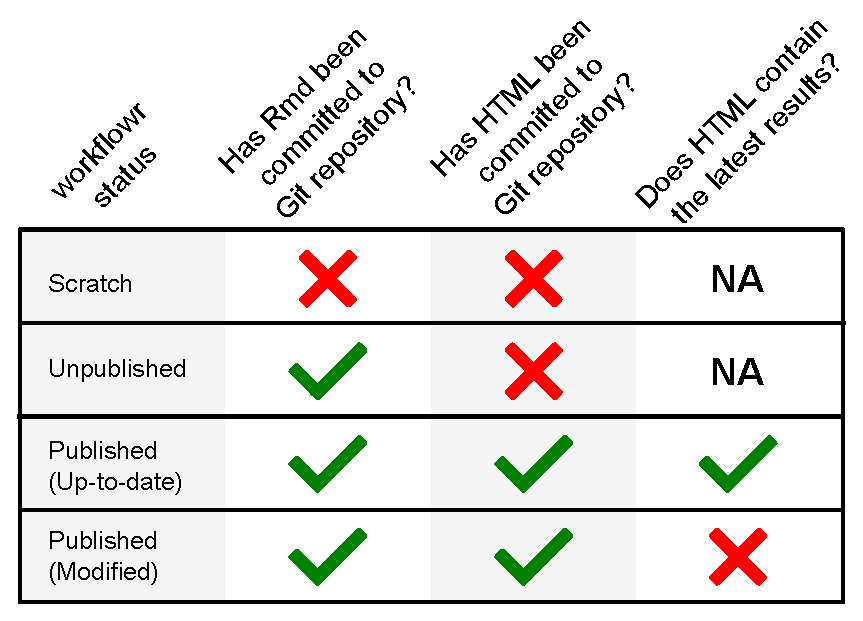
\includegraphics[width=0.8\textwidth]{figures/wflow-fig-3-v02.eps}

\cprotect\caption{\label{fig:versioned}

The workflowr package is an R Markdown-aware version control system. The
function \verb|wflow_status()| assigns a state to each R Markdown file in the
workflowr project based on its status in the Git repository's working
tree, and based on the Git status of the corresponding HTML file.

}

\end{figure}



\begin{figure}

\# Figure \ref{fig:reproducible}

\centering

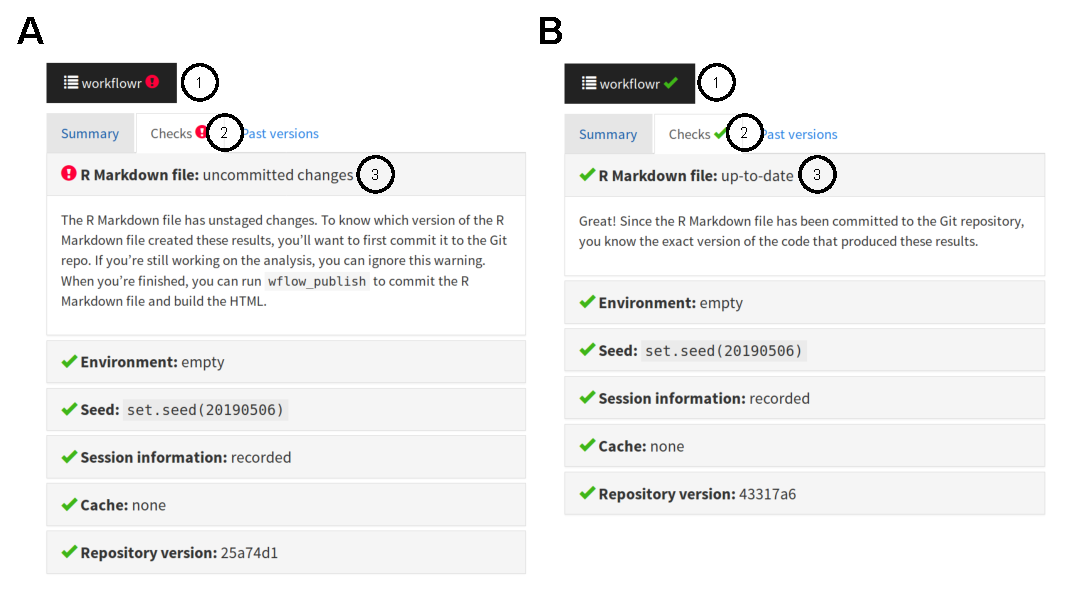
\includegraphics[width=0.8\textwidth]{figures/wflow-fig-4-v01.eps}

\cprotect\caption{\label{fig:reproducible}

The workflowr report summarizes the reproducibility checks inside the
results webpage. (A) A button is added to the top of each webpage.
Clicking on the button (1) reveals the full workflowr report with
multiple tabs. If any of the reproducibility checks have failed, a red
warning symbol (!) is shown. Clicking on the "Checks" tab (2) summarizes
the reproducibility checks, with icons next to each check indicating a
pass or failure. Clicking on an individual item (3) reveals a more
detailed description of the reproducibility check, with an explanation
of why it passed or failed. In (A), the R Markdown file contains changes
that have not yet been committed, failing one of the reproducibility
checks. (Uncommitted changes are acceptable during during active
development, but not acceptable when results are disseminated.) In this
case, a recommendation is given to run \verb|wflow_publish()| to fix the issue.
(B) If all the workflowr reproducibility checks pass, the workflowr
button shows a green checkmark ($\CheckmarkBold$), and clicking the
individual reproducibility checks (3) explains the importance of the
check.

}

\end{figure}

\subsubsection*{Sharing code and results: \verb|wflow_git_push()|}

The version-controlled website created by workflowr is self-contained,
so it can be hosted by most Web servers with little effort. Once the
website is available online, the code and results can be shared with
collaborators and colleagues by providing them with the website's URL.
Similarly, the workflowr repository can also serve as a companion
resource for a manuscript by referencing the website URL in the paper.

Since a workflowr project is also a Git repository, the most convenient
way to make the website available online is to use a Git hosting service
such as GitHub or GitLab. Since GitHub and GitLab are some of the most
widely used services, the workflowr package includes two functions,
\verb|wflow_use_github()| and \verb|wflow_use_gitlab()|, to simplify the tedious
process of setting up GitHub or GitLab for a workflowr project. Once a
user has created a Git repository on one of these online platforms, the
project can be uploaded to the remote service using \verb|wflow_git_push()|.
(Note that there is a companion function \verb|wflow_git_pull()| which would
only be used when multiple people are collaborating on a workflowr
project, or when project is being updated from multiple computers.)

One of our aims in integrating these website features into workflowr is
to make the version control features of a workflowr project accessible
to others without them having to execute a single line of code, or run
any program from the command-line shell; in addition to the
reproducibility report, workflowr automatically embeds links to past
versions of the R Markdown file, the corresponding results webpage, and
any figure files. For example, if a collaborator would like to download
a version of a figure that was generated from a set of results that was
generated several months ago, this can be done by navigating the links
on the workflowr website.

\subsubsection*{Installation}

The workflowr software is available on CRAN and can be downloaded by
simply running \verb|install.packages("workflowr")| in R. workflowr
works with R versions 2.3.5 or later, and it can be installed on any
major platform that is also supported by R (Linux, macOS, Windows). It
is regularly tested on all major operating systems via several
Continuous Integration services (AppVeyor, CircleCI, Travis CI). It is
also regularly tested by CRAN using machines running Debian GNU/Linux,
Fedora, macOS, Solaris and Windows.

Because workflowr uses the rmarkdown package to build the HTML pages, it
requires the document conversion software pandoc to be installed. The
easiest way for R users to install pandoc is to install RStudio, as
pandoc is packaged with the RStudio distribution. Installating Git is
not required, but may be useful for occasional management of the Git
repository outside regular workflowr usage.

\subsubsection*{Customization}

workflowr projects are designed to be highly customizable. For example,
the look of the webpages can be customized via options provided by the
rmarkdown package. These options can be customized in the
\verb|analysis/_site.yml| configuration file. Additional settings
specific to workflowr, such as setting the seed for the pseudorandom
number generation, or setting the working directory for the R Markdown
files, can be controlled in the \verb|_workflowr.yml| file.

\subsection*{Implementation}

Here we give an overview of the workflowr package implementation and its operation. All workflowr commands can be invoked from R (or RStudio) so long as the working directory in R is set to the directory containing a workflowr project, or any subdirectory of a workflowr project (this is similar to how Git commands are invoked). To determine the workflowr project from a subdirectory, whenever a command is called from the R console, workflowr searches for the RStudio project file stored at the root of the project. This search is implemented using the rprojroot R package. (The RStudio project file is a required file, so if this file is deleted, the workflowr commands will fail.)

\subsubsection*{Organizing files: \verb|wflow_start()|}

The function \verb|wflow_start()| populates the project directory using
predefined template files. It uses the glue R package to insert relevant
variables, e.g., the name of the project, directly into the newly
created files.

\subsubsection*{Generating the results reproducibly: \verb|wflow_build()|}

The \verb|wflow_build()| function generates a responsive website from a
collection of R Markdown files. It builds on the \verb|render_site()| function
from the rmarkdown package. Function \verb|render_site()| in turn builds on the
Bootstrap framework to create a responsive website with a navigation
bar. This includes downloading and linking to the required CSS and
JavaScript files. The website settings, such as the labels and URLs
included in the navigation bar, can be adjusted in the
\verb|analysis/_site.yml|configuration file. Like other R packages such
as bookdown that extend rmarkdown, workflowr provides a custom site
generator in function \verb|wflow_site()| that alters the website generation
process. For example, one change to this process is is that the
generated website files (HTML, CSS, JavaScript) are moved instead of
copied from \verb|analysis/| to \verb|docs/|, which . This reduces
unncessary duplication of files.

In the rmarkdown package, the rendering of webpages from R Markdown
files is controlled using function \verb|html_document()|. Workflowr provides
an analgous function, \verb|wflow_html()|, which extends \verb|html_document()|, and
allows for customization of the and the reproducibility checks.
Therefore, all features implemented in rmarkdown (e.g., code chunk
folding, generating a table of contents from the section headings) are
inherited by \verb|wflow_html()|.

Most of the workflowr content is added as a preprocessing step prior to
executing the R code in the R Markdown file. To do this, \verb|wflow_html()|
copies the original R Markdown file to a temporary directory, adds the
additional content, then executes the code. The content embded into the
R Markdown includes code chunks such as R code at the start of the file
that calls set.\verb|seed()| and R code toward the end of the file that calls
sessionI\verb|nfo()|, and inline HTML for elements such as the workflowr report
and links to previous versions of figures. There is also a brief
postprocessing step to incorporate additional HTML, CSS and JavaScript
elements needed to display the workflowr elements added in the
preprocessing step. This postprocessing is done when pandoc converts the
generated markdown to the final webpage.

The process for embedding links to past versions of files --- that is,
files added to previous commits in a Git repository --- requires some
additional explanation. Links to past versions are only included if the
user has set up a remote repository hosted by GitHub and GitLab.
Clicking a link to a past revsion of an R Markdown file (or figure file)
in a Web browser will load a webpage displaying the R Markdown source
code (or figure file) as it is saved in the given commit. For past
versions of the webpages, we use an independent service raw.githack.com,
which displays the HTML file in the browser like any other webpage,
whereas GitHub and GitLib shows the HTML code.

The settings in \verb|analysis/_site.yml| are passed to function
\verb|html_document()| in the rmarkdown package. The settings in
\verb|_workflowr.yml| are read by \verb|wflow_html()|; see help(wflow_html) for
a full documentation on all workflowr settings that can be customized in
this file. For example, the default function used to record the session
information at the bottom of each webpage, sessionI\verb|nfo()|, can be
overridden by adding a line to this YAML file that starts with
``sessioninfo:'' (e.g., the function from the devtools package could be
used instead by setting \verb|sessioninfo: devtools::session_info().

\verb|wflow_build()| creates a new R session to execute the code. This is
implemented using the R package callr. The workflowr package can be
configured to execute the R Markdown files in a different directory from
where they are saved. This execution directory is controlled by the
rmarkdown option \verb|knit_root_dir|, which is set in \verb|
_workflowr.yml| and read by \verb|wflow_html()| before executing the code. By
default, new projects execute the R Markdown code chunks in the root
directory.

\subsubsection*{Keeping track of the project's development: \verb|wflow_publish()|}

The workflowr functions use the R package git2r to run Git commands. The
git2r package is a wrapper around libgit2, a minimal C implementation of
Git.

This sequence of Git commands, and other operations, are executed behind
the scenes so that the user need only make a simple call to
\verb|wflow_publish()|. We have also implemented many checks and extensive
error handling to make sure that the Git repository and R environment
are in an acceptable state for committing the results. And when there
are issues that prevent commiting of results workflowr provides guidance
on how to fix them.

\subsubsection*{Checking in on the project's development: \verb|wflow_status()|}

The \verb|wflow_status()| function checks the status of each R Markdown file in
the project by comparing the state of the file in the Git repository's
working tree against the Git status of the corresponding HTML file. In
Git terminology, a “scratch” R Markdown file in a workflowr project is
an uncommitted file in a Git repository; “unpublished” means that the R
Markdown file is committed to the Git repository but the corresponding
HTML is not; a "published" R Markdown file and its HTML file are both
committed to the Git repository; and a "modified" R Markdown file has
changes --- these changes can be unstaged, staged, or committed --- that
were made since the last time the corresponding HTML file was committed
(Figure \ref{fig:versioned}).

\subsubsection*{Sharing the code and results: \verb|wflow_git_push()|}

o use \verb|wflow_git_push()|, the git remote must first be configured. The
user can configure the remotes manually using the git remote subcommand
or using \verb|wflow_git_remote()|. Alternatively, the workflowr package
provides two functions, \verb|wflow_use_github()| and \verb|wflow_use_gitlab()|, to
simplify the creation and configuration of remote repositories hosted on
GitHub and GitLab. These two convenience functions also add a navigation
bar link with the URL of the remote source code repository. The
\verb|wflow_use_gitlab()| function takes the additional setup of activating the
GitLab Pages by creating a file .gitlab-ci.yml with the proper
configuration. (GitHub Pages must be set up manually because there is
currently no way to do this automatically via the GitHub API.).

\subsubsection*{Installation of workflowr and software dependencies}

Distribution and installation of the workflowr package is managed by the
Comprehensive R Archive Network (CRAN). The one software requirement
that is not automatically installed on most systems is pandoc.
Fortunately, pandoc comes bundled with RStudio, so users do not need to
install pandoc separately as long as they install workflowr from
RStudio. Alternatively, if R is used instead of RStudio, pandoc is
available for download via popular package managers such as Homebrew and
Anaconda. Users do not need to install Git; workflowr uses the
cross-platform C library libgit2, which is interfaced to R via the R
package git2r.


\section*{Use cases} 

workflowr was officially released on CRAN in April 2018. As of July
2019, it has been downloaded from CRAN over 7,000 times, and it has been
adopted by many researchers to collaborate on research projects and
develop project websites to accompany research papers. Here we highlight
some successful examples.

\subsection*{REPOSITORIES FOR RESEARCH PROJECTS}

HUMAN DERMAL FIBROBLAST CLONALITY PROJECT

https://davismcc.github.io/fibroblast-clonality

A workflowr project accompanying a scientific paper on computational
methods for decoding the clonal substructures of somatic tissues from
DNA sequencing data \cite{McCarthy2018}. The webpages describe how to
reproduce the data processing and analysis, along with the outputs and
plots obtained by running the code.

CHARACTERIZING AND INFERRING QUANTITATIVE CELL CYCLE PHASE IN
SINGLE-CELL RNA-SEQ DATA ANALYSIS

https://github.com/jdblischak/fucci-seq

A workflowr project supporting a paper on measuring cell cycle phase and
gene expression levels in human induced pluripotent stem cells
\cite{Hsiao2019}. The repository contains the processed data and code
implementing the analyses, and the full results can be browsed in the
website.

FLEXIBLE STATISTICAL METHODS FOR ESTIMATING AND TESTING EFFECTS IN
GENOMIC STUDIES WITH MULTIPLE CONDITIONS

https://github.com/stephenslab/gtexresults

A workflowr project containing the code and data used to produce the
results on the GTEx data set that were presented in \cite{Urbut2018}.

INVESTIGATIONS ON "TRUNCATED ADAPTIVE SHRINKAGE"

https://github.com/LSun/truncash

A workflowr project a Ph.D. student created to keep track of his
investigations into controlling false discoveries in the presence of
correlation and heteroskedastic noise. This repository illustrates the
use of workflowr as a scientific notebook --- the webpages contain
written notes, mathematical equations, source code, and the outputs
generated from running the code.

\subsection*{REPOSITORIES FOR COURSES}

STANFORD STATS 141—BIOSTATISTICS

https://xiangzhu.github.io/stanford-stats141

A workflowr website for the Biostatistics course taught at Stanford. The
website includes working R examples, homework, the course syllabus and
other course materials.

SINGLE-CELL RNA-SEQ WORKSHOP

https://github.com/crazyhottommy/scRNA-seq-workshop-Fall-2019

A workflowr website for a workshop on analysis of single-cell RNA-seq
data offered by the Harvard Faculty of Arts and Sciences Informatics
group as part of a two-week long bioformatics course. The R examples
demonstrate use of several bioinformatics packages such as Seurat and
msigdbr for preparation and analysis of single-cell RNA-seq data sets.

INTRODUCTION TO GIS IN R

https://github.com/annakrystalli/intro-r-gis

A workflowr website for a workshop given at the 2018 Evolutionary
Biology Conference. The website includes working R demonstrations, setup
instructions, and exercises.

\section*{Summary}

Our main aim in developing workflowr is to lower barriers to open and
reproducible code. The R package is straightfoward to install, easy to
learn and highly customizable.

The core functionality has been stable and will continue to be. In the
future, we plan to implement the following enhancements:

\begin{itemize}

\item Provide documentation and helper functions to support hosting the
workflowr website on additional platforms. Because it is a static
website, it could be hosted on many different platforms such as GitLab,
Netlify, Heroku, etc.

\item Create a centralized website for registering and sharing workflowr
projects. In order to better promote open science, we would like to make
it easier for other interested researchers to discover existing
workflowr projects.

\item Implement basic support for small pipelines, including management
of code and file dependencies. Currently the only way to have workflowr
execute R Markdown files in a specific order is to name them in
alphanumeric order. In the future, we plan to make it possible to
specify which R Markdown files depend on each other. However, since it
will still be focused only on R Markdown files, users will still be
encouraged to use dedicated pipeline software to build complex data
analysis pipelines.

\end{itemize}

While workflowr aims to facilitate reproducible research, it is of
course not foolproof. Major limitations include 1) versioning of large
data files, 2) managing the computational environment, and 3) willful
tampering. The workflowr package ensures that each HTML results file was
created from a specific, known version of the corresponding R Markdown
file, which is critical for reproducibility. However, if any imported
data files are not versioned by Git (or are out-of-date), then the
results will not be reproducible. This is mainly an issue for large data
files. Users are recommended to use Git LFS or similar software to
version large data files. Managing software dependencies is complex, and
there exist many solutions ranging from language-specific package
managers (e.g. packrat) to operating-system-level virtualization (e.g.
Docker). Instead of prescribing one solution over others, the workflowr
package simply records the session information that produces each
result, and otherwise leaves each user to decide how best to manage this
complexity. Lastly, the development history recorded by Git can be
edited. Thus while useful for transparency, it cannot be considered an
immutable record (e.g. like that provided by a blockchain).


\section*{Data availability}

Not applicable.


\section*{Software availability}

The workflowr software is open source and available from these URLs:

\begin{enumerate}

\item CRAN: \url{https://cran.r-project.org/package=workflowr}

\item Source code: \url{https://github.com/jdblischak/workflowr}

\item Documentation and tutorials:
\url{https://jdblischak.github.io/workflowr/}

\item Zenodo: \url{https://zenodo.org/badge/latestdoi/75893305}

\item License: \href{https://choosealicense.com/licenses/mit}{MIT}

\end{enumerate}


\section*{Author Contributions}

JDB: Conceptualization, Software

PC: Software

MS: Conceptualization, Funding Acquisition, Supervision


\section*{Competing interests}

No competing interests were disclosed.


\section*{Grant information}

This work was supported by the Gordon and Betty Moore Foundation [Grant
number \#4559].

The funders had no role in study design, data collection and analysis,
decision to publish, or preparation of the manuscript.


\section*{Acknowledgments}

We thank the workflowr
\href{https://github.com/jdblischak/workflowr/graphs/contributors}{contributors}
for helping improve the package. We are also grateful for the many
workflowr users for testing the package and providing feedback---thanks
especially to \href{https://github.com/LSun}{Lei Sun},
\href{https://github.com/xiangzhu}{Xiang Zhu},
\href{https://github.com/NKweiwang}{Wei Wang}, and many other members of
the Stephens lab, past and present. We also acknowledge the authors and
contributors of the many great open source packages that the workflowr
package builds on. R packages particularly critical to workflowr's
implementation are
\href{https://cran.r-project.org/web/packages/git2r/index.html}{git2r},
\href{https://github.com/yihui/knitr}{knitr} and
\href{http://rmarkdown.rstudio.com/}{rmarkdown}.

{\small\bibliographystyle{unsrtnat}

\bibliography{references}}

\end{document}
